%
% eScience 2013
%
\documentclass[final]{IEEEtran}
\hyphenation{op-tical net-works semi-conduc-tor}

\usepackage{makeidx}  % allows for indexgeneration
\usepackage{algorithm,algpseudocode}
\usepackage{graphicx}
\usepackage{float}
\usepackage{subcaption}
\captionsetup{compatibility=false}
\usepackage{wrapfig}
\usepackage{array}
\usepackage{cite}

\begin{document}

\title{Balanced Task Clustering in Scientific Workflows}


\author{
  \IEEEauthorblockN{
    Weiwei Chen\IEEEauthorrefmark{1}, 
    Rafael Ferreira da Silva\IEEEauthorrefmark{3}, 
    Ewa Deelman\IEEEauthorrefmark{1},
    Rizos Sakellariou\IEEEauthorrefmark{4}\\
  }
  \IEEEauthorblockA{
     \IEEEauthorrefmark{1}University of Southern California, Information Sciences Institute, Marina Del Rey, CA, USA\\
     \{wchen,deelman\}@isi.edu \\
  }
  \IEEEauthorblockA{
    \IEEEauthorrefmark{3}University of Lyon, CNRS, INSERM, CREATIS, Villeurbanne, France\\
    rafael.silva@creatis.insa-lyon.fr \\
  }
  \IEEEauthorblockA{
    \IEEEauthorrefmark{4}University of Manchester, School of Computer Science, Manchester, U.K.\\
    rizos@cs.man.ac.uk
  }
}

\maketitle

\begin{abstract}
Scientific workflows can be composed of many fine computational granularity tasks. The runtime of these tasks may be shorter than the duration of system overheads, for example, when using multiple resources of a cloud infrastructure. Task clustering is a runtime optimization technique that merges multiple short tasks into a single job such that the scheduling overhead is reduced and the overall runtime performance is improved. However, existing task clustering strategies only provide a coarse-grained approach that relies on an over-simplified workflow model. In our work, we examine the reasons that cause Runtime Imbalance and Dependency Imbalance in task clustering. Next, we propose quantitative metrics to evaluate the severity of the two imbalance problem respectively. Furthermore, we propose a series of task balancing methods to address these imbalance problems. Finally, we analyze their relationship with the performance of these task balancing methods. A trace-based simulation shows our methods can significantly improve the runtime performance of two widely used workflows compared to the existing implementation of task clustering.

\begin{IEEEkeywords}
Scientific workflow, data locality, load balance, task clustering
\end{IEEEkeywords}
\end{abstract}


\IEEEpeerreviewmaketitle


% Section
\section{Introduction}

Many computational scientists develop and use large-scale, loosely-coupled applications that are often structured as scientific workflows, which consist of many computational tasks with data dependencies between them. Although the majority of the tasks within these applications are often relatively short running (from a few seconds to a few minutes), in aggregate they represent a significant amount of computation and data~\cite{LIGO}. When executing these applications on a multi-machine distributed environment, such as the Grid or the Cloud, significant system overheads may exist and may adversely slowdown the application performance~\cite{Chen}. To minimize the impact of such overheads, task clustering techniques~\cite{Muthuvelu:2005:DJG:1082290.1082297,4493929,Muthuvelu2010,Muthuvelu2013170,keat-2006,ang-2009,4958835,Singh:2008:WTC:1341811.1341822,europar-granularity} have been developed to group \emph{fine-grained} tasks into \emph{coarse-grained} tasks so that the number of computational activities is reduced and their computational granularity is increased thereby reducing the (mostly scheduling related) system overheads~\cite{Chen}.
%Existing task clustering strategies have demonstrated their effect in some scientific workflows such as CyberShake \cite{Rynge1} and LIGO \cite{LIGO}. 
However, there are several challenges that have not yet been addressed.

In a scientific workflow, tasks within a level may have different runtimes. Merging tasks without considering the runtime variance may cause load imbalance, i.e., some clustered jobs may be composed by short tasks while others by long tasks. This imbalance delays the release of tasks from the next level, penalizing the workflow execution with an overhead produced by the use of inappropriate task clustering strategies~\cite{Chen2013}.
A common technique to handle load imbalance is overdecomposition~\cite{Lifflander}.
%The first challenge users face when executing workflows is task runtime variation. Tasks may have diverse task runtimes and such diversity may cause some load imbalance. The last completed task among a given set of tasks essentially controls the release of next set of tasks. A popular technique in workload studies  to address the load balancing challenge is overdecomposition \cite{Lifflander}.
This method decomposes computational work into medium-grained balanced tasks. Each task is coarse-grained enough to enable efficient execution and reduce scheduling overheads, while being fine-grained enough to expose significantly higher application-level parallelism than that is offered by the hardware. 

Data dependencies between workflow tasks play an important role when clustering tasks within a level. A data dependency means that there is a data transfer between two tasks (output data for one and input data for the other). Grouping tasks without considering these dependencies may lead to data locality problems where output data produced by parent tasks are poorly distributed. Thus, data transfer times and failures probability increase.
Therefore, we claim that data dependencies of subsequent tasks should be considered.

%The second challenge has to do with the complex data dependencies within a workflow. A data dependency means there is a data transfer between two tasks (input data for one task and output data for the other). Merging tasks that have no intermediate data between them seems safe at the first sight. However, the subsequent tasks that rely on the output data that their parent tasks produce may suffer a data locality problem since data may be distributed poorly and the data transfer time is increased. Therefore, we claim that it is necessary to consider the data dependencies with subsequent tasks (not only child tasks). 
%Generally speaking, tasks without intermediate data between them should be distributed inside a cluster in order to fully utilize the computational capabilities. 

%These challenges constitute the imbalance problem (runtime imbalance or dependency imbalance), which refers to a scenario that some clustered jobs are postponed for execution caused by unavailable data, overloaded resources, or system constraints due to inefficient task clustering. 

In this work, we generalize these two challenges (Runtime Imbalance and Dependency Imbalance) to the generalized load balance problem. We introduce a series of balancing methods to address these challenges as our first contribution. A performance evaluation study shows that they can significantly reduce the imbalance problem.

%It means that the execution of workflows suffers from significant overheads (unavailable data, overloaded resources, or system constraints) due to inappropriate task clustering and job execution. To solve the imbalance problem, we introduce a series of balancing methods to address these two challenges respectively as our first contribution. The performance evaluation shows that they can significantly reduce the imbalance problem. 

However, there is a tradeoff between runtime and data dependency balancing. For instance, 
%However, what makes this problem challenging is that the solutions are usually conflicting. For example, 
balancing runtime may aggravate the Dependency Imbalance problem, and vice versa. A quantitative measurement of workflow characteristics is required to serve as a criterion to select and balance these solutions. To achieve this goal, we propose a series of metrics that reflect the internal structure (in terms of runtime and dependency) of the workflow as our second contribution. 

In particular, we provide a novel approach to capture these metrics. Traditionally, there are two approaches to improve the performance of task clustering. The first one is a top-down approach \cite{6217508} that represents the clustering problem as a global optimization problem and aims to minimize the overall runtime of a workflow. However, the complexity of solving such an optimization problem does not scale well since they use genetic algorithms. The second one is a bottom-up approach~\cite{Muthuvelu:2005:DJG:1082290.1082297,4958835} that only examines free tasks to be merged and optimizes the clustering results locally. In contrast, our work extends these solutions to consider the neighboring tasks including siblings, parents, and children because such a family of tasks has strong connections between them. 

Our third contribution is an analyze of the quantitative metrics and balancing methods. These metrics characterize the workflow imbalance problem. A balancing method, or a combination of those, is selected through the comparison of the relative values of these metrics.

%The third contribution we make is that we analyze and connect the performance of these metrics and balancing methods. These quantitative metrics indicate which type of imbalance problem a workflow is more likely to suffer from. Comparing the relative values of these metrics informs the selection of a balancing method or a combination of these methods. 

%In this paper, we improve the runtime balance of task clustering to complete large-scale and fine-grained workflows on distributed environments efficiently. This paper is organized as follows. Section 2 provides research work related to balanced clustering. Section 3 analyzes the model of balanced clustering and explains the design of our heuristics and algorithms. We conclude in Section 5. We evaluate our balanced clustering in Section 4. Section 5 discusses limitations and extensions of balanced clustering.
%

To the best of our knowledge, this study is the first example of task granularity control that considers runtime variance and data dependency. The next Section gives an overview of the related work, Section~\ref{sec:model} presents our workflow and execution environment models, Section~\ref{sec:heuristics} details our heuristics and algorithms, Section~\ref{sec:experiments} reports experiments and results, and the paper closes with a discussion and conclusions.


% Section
\section{Related Work}

The low performance of \emph{fine-grained} tasks is a common problem in widely distributed platforms where the scheduling overhead and queuing times are high, such as Grid and Cloud systems. Several works have addressed the control of task granularity of bag of tasks. For instance, Muthuvelu et al.~\cite{Muthuvelu:2005:DJG:1082290.1082297} proposed a clustering algorithm that groups bag of tasks based on their runtime---tasks are grouped up to the resource capacity. Later, they extended their work~\cite{4493929} to determine task granularity based on task file size, CPU time, and resource constraints. Recently, they proposed an online scheduling algorithm~\cite{Muthuvelu2010,Muthuvelu2013170} that groups tasks based on resource network utilization, user's budget, and application deadline. Ng et al.~\cite{keat-2006} and Ang et al.~\cite{ang-2009} introduced bandwidth in the scheduling framework to enhance the performance of task scheduling. Longer tasks are assigned to resources with better bandwidth. Liu and Liao~\cite{4958835} proposed an adaptive fine-grained job scheduling algorithm to group fine-grained tasks according to processing capacity and bandwidth of the current available resources. Although these techniques significantly reduce the impact of scheduling and queuing time overhead, they are not applicable to scientific workflows, since data dependencies are not considered.

Task granularity control has also been addressed in scientific workflows. For instance, Singh et al.~\cite{Singh:2008:WTC:1341811.1341822} proposed a level- and label-based clustering. In level-based clustering, tasks at the same level can be clustered together. The number of clusters or tasks per cluster are specified by the user. In the label-based clustering, the user labels tasks that should be clustered together. Although their work considers data dependency between workflow levels, it is done manually by users, which is prone to errors. Recently, Ferreira da Silva et al.~\cite{europar-granularity} proposed task grouping and un-grouping algorithms to control workflow task granularity in a non-clairvoyant and online context. Their work significantly reduced scheduling and queuing time overheads, but did not consider data dependencies.


%\textbf{Workflow Management Systems} (WMS) such as Askalon \cite{Fahringer}, Taverna \cite{Oinn}, and Pegasus \cite{Deelman} are designed to run scientific workflows on distributed environments. DAGs (Directed Acyclic Graph) and other task graph representations are widely used as the programming model for many parallel applications because it is effective in expressing and optimizing irregular computations. 
%Moreover, algorithms expressed as DAGs have the potential to alleviate the user from focusing on the architectural issues, while allowing the engine to extract the best performance from the underlying architecture. 


%\textbf{Load Balance}. 
A plethora of balanced scheduling algorithms have been developed in the networking and operating system domains. Many of these schedulers have been extended to the hierarchical setting. Lifflander et al.~\cite{Lifflander} proposed to use work stealing and a hierarchical persistence-based rebalancing algorithm to address the imbalance problem in scheduling. Zheng et al.~\cite{Zheng} presented an automatic hierarchical load balancing method that overcomes the scalability challenges of centralized schemes and poor solutions of traditional distributed schemes. There are other scheduling algorithms~\cite{Braun2001} (e.g. list scheduling) that indirectly achieve load balancing of workflows through makespan minimization. However, the benefit that can be achieved through traditional scheduling optimization is limited by its complexity. The performance gain of task clustering is primarily determined by the ratio between system overheads and task runtime, which is more substantial in modern distributed systems such as Clouds and Grids. 

%Compared to them, our work aims to create clustered jobs that have an even distribution in the job runtime and dependency. 
%even though the distribution of task runtime is not even.  
%In our case, since we assume resources are homogeneous, the load balance in scheduling is not a major concern and thus we focus on the task clustering problem. 

%\textbf{Overhead Analysis}. Overhead analysis \cite{Prodan}\cite{Chen} is a topic of great interest in the grid community. Stratan \cite{Stratan} evaluates workflow engines including DAGMan/Condor and Karajan/Globus in a real-world grid environment. Sonmez \cite{Sonmez} investigated the prediction of the queue delay in grids and assessed the performance and benefit of predicting queue delays based on traces gathered from various resource and production grid environments. Prodan \cite{Prodan} offers a grid workflow overhead classification and a systematic measurement of overheads. Our prior work \cite{Chen} further investigated the major overheads and their relationship with different optimization techniques. In this paper, we classify the system overheads to clustering delay and scheduling overheads, which have different influence on the performance of task clustering \cite{Chen1}. 

%Section
\section{Model and Design}
\label{sec:model}


A workflow is modeled as a Directed Acyclic Graph (DAG). Each node in the DAG often represents a workflow task ($t$), and the edges represent dependencies between the tasks that constrain the order in which the tasks are executed. Dependencies typically represent data-flow dependencies in the application, where the output files produced by one task are used as inputs of another task. Each task is a program and a set of parameters that need to be executed. Fig.~\ref{fig:odag} (left) shows an illustration of a DAG composed by four tasks. This model fits several workflow management systems such as Pegasus~\cite{Deelman:2005:PFM:1239649.1239653}, Askalon~\cite{Fahringer:2005:ATS:1064323.1064331}, and Taverna~\cite{Oinn:2006:TLC:1148437.1148448}.

\begin{figure}[htb]
	\centering
	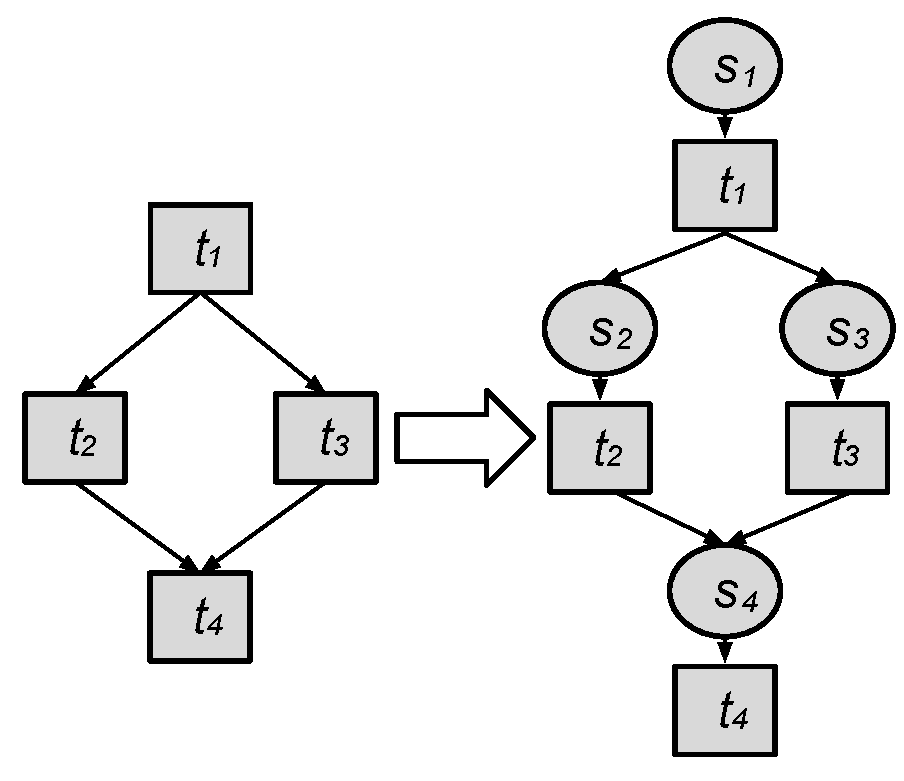
\includegraphics[width=0.7\linewidth]{figure/odag.pdf}
	\captionof{figure}{Extending DAG to o-DAG.}
	\label{fig:odag}
	\vspace{-10pt}
\end{figure}

%I may need to keep them here since I need to introduce the o-DAG model and it is execution dependent. 
Fig.~\ref{fig:system} shows a typical workflow execution environment. The submit host prepares a workflow for execution (clustering, mapping, etc.), and worker nodes, at an execution site, execute jobs individually. The main components are introduced below:

\begin{figure}[htb]
\centering
  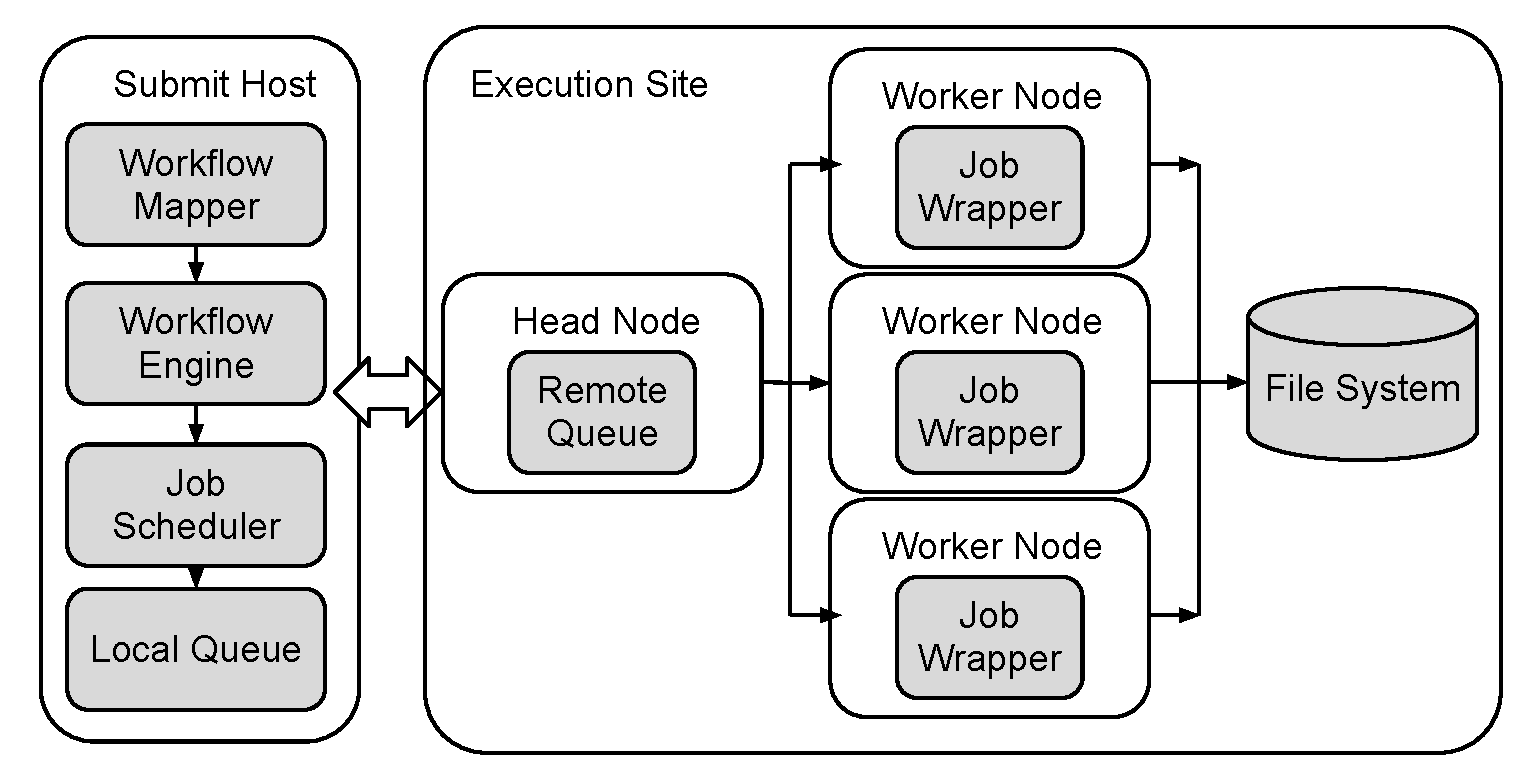
\includegraphics[width=0.95\linewidth]{figure/execution_vertical.pdf}
  \caption{A workflow system model.}
  \label{fig:system}
  \vspace{-10pt}
\end{figure}

\paragraph{Workflow Mapper} generates an executable workflow based on an abstract workflow provided by the user or workflow composition system. It also restructures the workflow to optimize performance and adds tasks for data management and provenance information generation. In this work, workflow mapper is particularly used to merge small tasks together into a job such that system overheads are reduced, which is called \textbf{Task Clustering}. A job is a single execution unit in the workflow execution systems and it may contain one or more tasks. 

\paragraph{Workflow Engine} executes jobs defined by the workflow in order of their dependencies. Only jobs that have all their parent jobs completed are submitted to the Job Scheduler. Workflow Engine relies on the resources (compute, storage, and network) defined in the executable workflow to perform the necessary actions. The time period when a job is free (all of its parents have completed successfully) to when it is submitted to the job scheduler is denoted the workflow engine delay. The workflow engine delay is usually configured by users to assure that the entire workflow scheduling and execution system is not overloaded. 

\paragraph{Job Scheduler and Local Queue} manage individual workflow jobs and supervise their execution on local and remote resources. The time period when a task is submitted to the job scheduler to when the task starts its execution in a worker node is denoted the queue delay. It reflects both the efficiency of the job scheduler and the resource availability. 

\paragraph{Job Wrapper} extracts tasks from clustered jobs and executes them at the worker nodes. The clustering delay is the  elapsed time on the extraction process.

In this work, we extend the DAG model to be overhead aware (o-DAG). System overheads play an important role in workflow execution and constitute a major part of the overall runtime when tasks are poorly clustered. Fig.~\ref{fig:odag} shows how we augment a DAG to be an o-DAG with the capability to represent scheduling overheads ($s$) such as workflow engine delay and queue delay. This classification of scheduling overheads is based on our prior study on workflow analysis~\cite{Chen}. 



%However, we still use DAGs in some cases to save space without causing misleading (such as in Fig.~\ref{fig:pipeline}). 

With an o-DAG model, we can explicitly express the process of task clustering. For instance, in Fig.~\ref{fig:hc}, two tasks $t_1$ and $t_2$, without data dependency between them, are merged into a clustered job $j_1$. A job $j$ is a single execution unit composed by one or multiple task(s). Job wrappers are commonly used to execute clustered jobs, but they add a overhead denoted the clustering delay $c$. 
Clustering delay measures the difference between the sum of the actual task runtimes and the job runtime seen by the job scheduler. 
%The cause of clustering delay is usually the use of a job wrapper to execute a clustered job. 
%The job wrapper takes some time to extract the list of tasks and to launch them.
%With o-DAG model, we can explicitly express the process of task clustering. For example, in Fig~\ref{fig:hc}, two tasks $t_1$ and $t_2$ without data dependency between them are merged into a clustered job $j_1$. 
%Scheduling overheads ($s$) are reduced but clustering delay is added. 
After horizontal clustering, $t_1$ and $t_2$ in $j_1$ can be executed in sequence or in parallel, if supported. In this paper, we consider sequential executions only. Given a single resource, the overall runtime for the workflow in Fig.~\ref{fig:hc} (left) is $runtime_1=s_1+t_1+s_2+t_2$ , and the overall runtime for the clustered workflow in Fig.~\ref{fig:hc} (right) is $runtime_2=s_1+c_1+t_1+t_2$.  $runtime_1 > runtime_2$ as long as $c_1 < s_2$, which is the case of many distributed systems since the clustering delay within an execution node is usually shorter than the scheduling overhead across different execution nodes.

\begin{figure}[htb]
\centering
 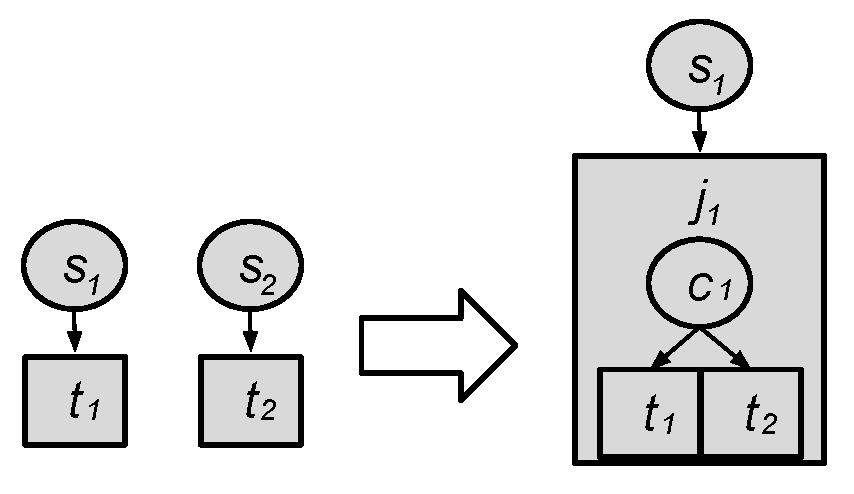
\includegraphics[width=0.65\linewidth]{figure/hc.pdf}
  \captionof{figure}{An Example of Task Clustering.}
  \label{fig:hc}
  \vspace{-10pt}
\end{figure}

%A more comprehensive analysis of system overheads is in \cite{Chen}.
%We then introduce two basic types of task clustering that are widely used in scientific workflows. 
%\textbf{Task Clustering}  is an optimization technique that merges fine-grained tasks into larger jobs to reduce the scheduling overhead and thereby the overall runtime is reduced as well. Specifically, Pegasus WMS \cite{Singh} supports horizontal clustering and label-based clustering. \textbf{Horizontal Clustering} (HC) merges tasks on the same level of the workflow. In their work, the level for a task is determined by doing a Breadth First Search of the underlying DAG. In contrast, we define the level of a task as the longest depth from the root task to this task (Depth First Search) because the longest depth controls the final release of this task. In label-based clustering, the user identifies tasks in the abstract workflow description that they want to execute as one cluster by associating labels with the tasks. Tasks associated with the same label are put into the same clustered job. However, these techniques are not aware of the data dependencies and expected runtime of tasks. 

Fig~\ref{fig:hc} shows a typical example of a Horizontal Clustering (HC) technique that groups tasks at the same horizontal level. In our work, we define the level of a task as the longest depth from the root task to this task because the longest depth controls the final release of this task. 
%Fig~\ref{fig:vc} shows another type of clustering called \textbf{Vertical Clustering} (VC) that aims to merge tasks at the same pipeline. A pipeline of tasks is a chain of tasks (such as $t_1$, $t_5$ and $t_9$ in Fig~\ref{fig:pipeline}) connected by data dependencies. Particularly any two connected tasks in a pipeline should have a one-to-one relationship, which means the parent task is the only parent of the children task and the children task is the only children of the parent task. 

%\begin{figure}[lh!]
%\centering
%  \includegraphics[height=0.5\linewidth]{figure/vc.png}
%  \captionof{figure}{Vertical Clustering}
%  \label{fig:vc}
%\end{figure}

In summary, an o-DAG representation allows the specification of high level system overhead details, which is more suitable than DAG models when clustering tasks.
% used in some previous work. 

\section{Balanced Clustering}
\label{sec:heuristics}

In this section we introduce the imbalance problem we are going to solve and we present metrics to quantitatively capture workflow characteristics, and methods to handle runtime and dependency imbalances.

%Figure 9 shows how we implement VC. Once we detect there exist a one-to-one relationship between two tasks (line 5), we merge them. Below we prove that VC is always beneficial and thereby it is always safe to perform VC. In Figure 10, $t_1$ is a parent of $t_2$ and VC merges them into a new job $j_1$. The overall makespan of the two tasks before clustering is $runtime_1=s_1+t_1+s_2+t_2$, and the overall makespan after clustering is $runtime_2=s_1+c_1+t_1+t_2$. 
%Similar to the discussion in Figure 3, we conclude that it is always beneficial (but not necessarily optimal) to perform vertical clustering because it may cause other imbalance problems to be shown below. VC is particularly useful when we have a Runtime Imbalance problem caused by dependencies with offspring tasks since we can merge tasks at the same pipeline and this problem is simplified to the Runtime Imbalance problem caused by child tasks. 

\subsection{Balanced Clustering Metrics}


%In this paper, we discuss two major imbalance problem: Runtime Imbalance and Dependency Imbalance:
%As already mentioned, in this paper, we discuss two imbalance problems:

\textbf{Runtime Imbalance} describes the difference of the task/job runtime of a group of tasks/jobs. In this work, we denote the \textbf{Horizontal Runtime Variance} ($HRV$) as the ratio of the standard deviation in task runtime to the average runtime of tasks/jobs at the same horizontal level of a workflow. At the same horizontal level, the job with the longest runtime often controls the release of the next level jobs. A high $HRV$ value means that the release of next level jobs has been delayed.
% Among all the types of Runtime Imbalance, we use two basic ones: \textbf{Horizontal Runtime Variance} ({\em HRV}) and \textbf{Pipeline Runtime Variance} ({\em PRV}). {\em HRV} is defined as the standard deviation of task/job runtime at the same horizontal level. At the same horizontal level, the job with the longest runtime often controls the release of next level jobs. 
Therefore, to improve runtime performance, it is meaningful to reduce the standard deviation of job runtime. Fig.~\ref{fig:rv} shows an example of four independent tasks $t_1$, $t_2$, $t_3$ and $t_4$ where task runtime of $t_1$ and $t_2$ is half of that of $t_3$ and $t_4$. In the approach of Horizontal Clustering (HC), a possible clustering result could be merging $t_1$ and $t_2$ into a clustered job and $t_3$ and $t_4$ into another. This approach results in imbalanced runtime, i.e., $HRV > 0$ (Fig.~\ref{fig:rv}-top). In contrast, a balanced clustering strategy should try its best to evenly distribute task runtime among jobs as shown in Fig.~\ref{fig:rv} (bottom). Generally speaking, a smaller \emph{HRV} means that the runtime of tasks at the same horizontal level is more evenly distributed and therefore it is less necessary to balance the runtime distribution. However, runtime variance is not able to describe how regular is the structure of the dependencies between the tasks.

\begin{figure}[htb]
	\centering
	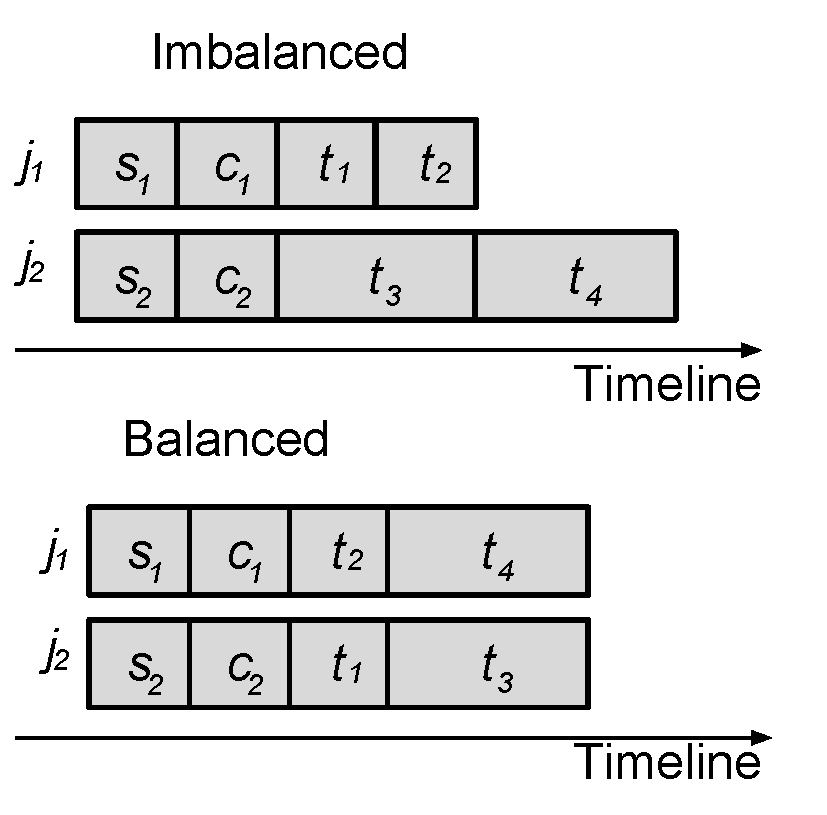
\includegraphics[width=0.6\linewidth]{figure/rv.pdf}
	\captionof{figure}{An Example of Runtime Variance.}
	\label{fig:rv}
	\vspace{-10pt}
\end{figure}

%For example, the {\em HRV} of the first level tasks in Fig~\ref{fig:dv} is the standard deviation of $t_1$, $t_2$, $t_3$, and $t_4$. 


%Pipeline Runtime Variance ({\em PRV}) is defined as the standard deviation of the cumulative runtime of pipelines. For example, the {\em PRV} of the four pipelines in Fig~\ref{fig:pipeline} is the standard deviation of ($t_1+ t_5 +t_9$), ($t_2+t_6+t_{10}$), ($t_3 +t_7+t_{11}$), and ($t_4+t_8+t_{12}$).

%\begin{minipage}[b]{0.3\textwidth}
%\centering
%  \includegraphics[width=0.8\linewidth]{figure/pipeline.png}
%  \captionof{figure}{Pipelines}
%  \label{fig:pipeline}
%\end{minipage}
%\end{figure}


%is the second reason why we need to use balanced clustering and it

\textbf{Dependency Imbalance} means that the task clustering at one horizontal level forces the tasks at the next level (or even subsequent levels) to have severe data locality problem and thus loss of parallelism. For example, in Fig.~\ref{fig:dv}, we show a two-level workflow composed by four tasks in the first level and two in the second. Merging $t_1$ with $t_2$ and $t_3$ with $t_4$ (imbalanced workflow in Fig.~\ref{fig:dv}) forces $t_5$ and $t_6$ to transfer files from two locations and wait for the completion of $t_1$, $t_2$, $t_3$, and $t_4$.  A balanced clustering strategy groups tasks that have the maximum number of child tasks in common. Thus, $t_5$ can start to execute as soon as $t_1$ and $t_3$ are completed, and so can $t_6$. To measure and quantitatively demonstrate the Dependency Imbalance of a workflow, we propose two  metrics: ($i$) Impact Factor Variance, and ($ii$) Distance Variance. 

\begin{figure}[htb]
	\centering
	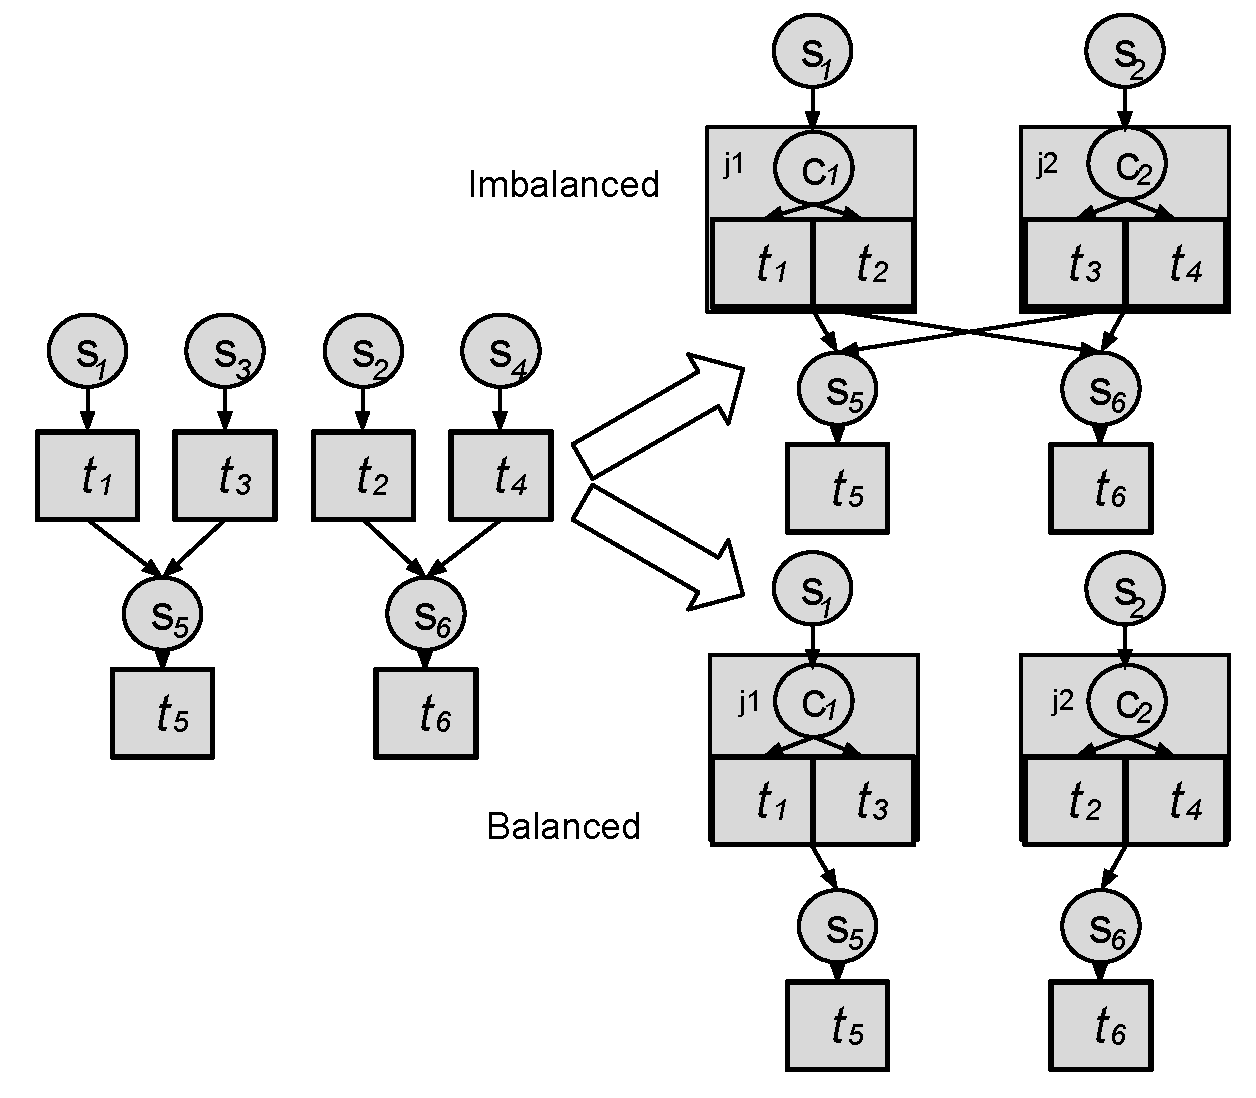
\includegraphics[width=\linewidth]{figure/dv.pdf}
	\captionof{figure}{An Example of Dependency Variance.}
	\label{fig:dv}
	\vspace{-10pt}
\end{figure}

We define the \textbf{Impact Factor Variance} ($IFV$) of tasks as the standard deviation of their impact factor. The intuition of Impact Factor is that we aim to capture the similarity of tasks/jobs in a graph by measuring their relative impact factor or importance to the entire graph. Intuitively speaking, tasks with similar impact factors should be merged together compared to tasks with different impact factors. Also, if all the tasks have similar impact factors, the workflow structure tends to be more 'even' or 'regular'. The \textbf{Impact Factor} ($IF$) of a task $t_u$ is defined as follows:

%We first define the \textbf{Impact Factor} ($IF$) of a task in a recursive way as below. 

\begin{equation}
	IF(t_u)=\sum_{t_v\in Child(t_u)}^{}\frac{IF(t_v)}{L(t_v)}
\end{equation}
where $Child(t_u)$ denotes the set of child tasks of $t_u$, and $L(t_v)$ the number of parent tasks of $t_v$. For simplicity, we assume the $IF$ of a workflow exit task (e.g. $t_5$ in Fig.~\ref{fig:dv}) as 1.0. For instance, consider the two workflows presented in Fig.~\ref{fig:hifv}. $IF$ for $t_1$, $t_2$, $t_3$, and $t_4$ are computed as follows:

\begin{eqnarray}
	\displaystyle  
	&IF(t_7 )=1.0, IF(t_6 )=IF(t_5 )=IF(t_7 )/2=0.5\nonumber  \\
	&IF(t_1 )=IF(t_2 )=IF(t_5 )/2=0.25\nonumber \\
	&IF(t_3 )=IF(t_4 )=IF(t_6 )/2=0.25\nonumber 
\end{eqnarray}
Thus, IFV($t_1$, $t_2$, $t_3$, $t_4$) = 0. In contrast, $IF$ for $t_1'$, $t_2'$, $t_3'$, and $t_4'$ are:

\begin{eqnarray}
	\displaystyle  
	&IF(t_7')=1.0, IF(t_6')=IF(t_5')=IF(t_1')=IF(t_7')/2=0.5\nonumber \\
	&IF(t_2')=IF(t_3')=IF(t_4')=IF(t_6')/3=0.17 \nonumber
\end{eqnarray}
Therefore, the $IFV$ value for {$t_1'$, $t_2'$, $t_3'$, $t_4'$} is 0.17, which means it is less regular than the workflow in Fig.~\ref{fig:hifv} (left). In this work, we use \textbf{HIFV} (Horizontal IFV) to indicate the $IFV$ of tasks at the same horizontal level. The time complexity of calculating all the $IF$ of a workflow with $n$ tasks is $O(n)$.  



\begin{figure}[htb]
	\centering
	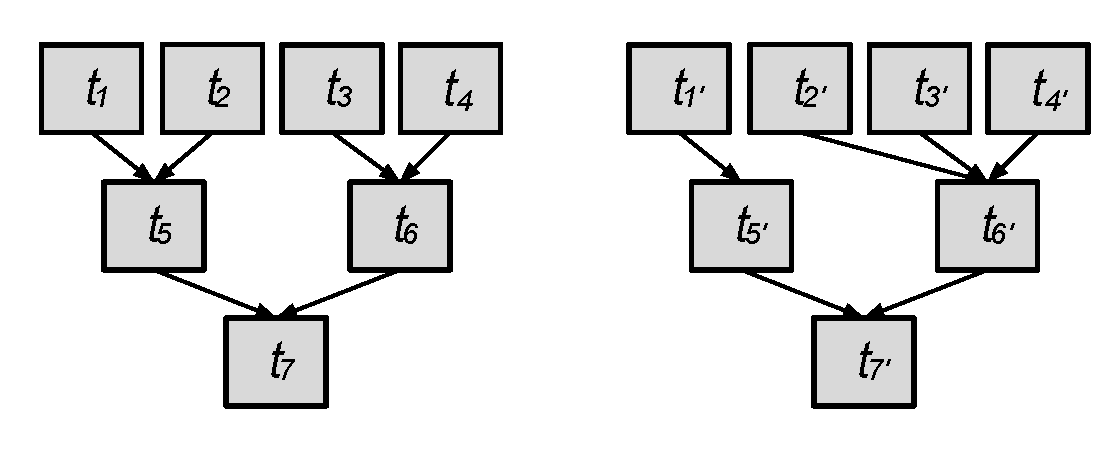
\includegraphics[width=0.85\linewidth]{figure/hifv.pdf}
	\captionof{figure}{Example of workflows with different data dependencies.}
	\label{fig:hifv}
	\vspace{-10pt}
\end{figure}
% In Fig~\ref{fig:hifv}, the left workflow should have a smaller Dependency Imbalance problem than the right workflow since the dependencies in the left figure are more repetitive and regular. We define the \textbf{Impact Factor Variance} ({\em IFV}) of tasks to be the standard deviation of their $IF$. Therefore, the {\em IFV} of {$t_1$, $t_2$, $t_3$, $t_4$} is 0. In contrast, for the workflow in Fig~\ref{fig:hifv} (Right), we have:

\textbf{Distance Variance} ($DV$) describes how `closely' tasks are to each other. The distance between two tasks/jobs is defined as the cumulative length of the path to their closest common successor. If they do not have a common successor, the distance is set to infinity. For a group of $n$ tasks/jobs, the distance between them is represented by a $n \times n$ matrix $D$, where an element $D(u,v)$ denotes the distance between a pair of tasks/jobs $u$ and $v$. For any workflow structure, $D(u,v)=D(v,u)$ and $D(u,u)=0$, thus we ignore the cases when $u \geq v$. Distance Variance is then defined as the standard deviation of all the elements $D(u,v)$ for $u<v$. The time complexity of calculating all the $D$ of a workflow with $n$ tasks is $O(n^2)$. 

Similarly, $HDV$ indicates the $DV$ of a group of tasks/jobs at the same horizontal level. For example, Table~\ref{tab:1} shows the distance matrices of tasks from the first level for both workflows of Fig.~\ref{fig:hifv} ($D_1$ for the workflow in the left and $D_2$ for the workflow in the right). $HDV$ for $t_1, t_2, t_3$, and $t_4$ is 1.03, and for $t_1', t_2', t_3'$, and $t_4'$ is 1.10. In terms of distance variance, $D_1$ is more `even' than $D_2$. Intuitively speaking, a smaller $HDV$ means the tasks at the same horizontal level are more equally 'distant' to each other and thus the workflow structure tends to be more 'evenly' and 'regular'. 

In conclusion, Runtime Variance and Dependency Variance offer a quantitative and comparable tool to measure and evaluate the internal structure of a workflow. 

%In next section, we will indicate how these metrics connect to the performance of different balancing methods. 

%Overhead is the another cause of the Runtime Imbalance problem. In our previous work [24], we have shown that overheads have diverse distribution and they have different influence on the overall runtime of workflows. In Figure 7, we show an example where the workflow engine checks two jobs at a working cycle and increases the workflow engine delay steadily in every working cycle. Merging tasks into four jobs may fully utilize the available resources. However, the increase in workflow engine delay may counteract the benefit we gain from task clustering. In such case, a balanced clustering strategy should try to merge tasks into as fewer jobs as possible. 

\begin{table}[htb]
	\footnotesize
	\centering
	\begin{tabular}{l|rrrr}
		$D_1$ & $t_1$ & $t_2$ & $t_3$ &$t_4$\\
		\hline
		$t_1$ & 0 & 2 & 4 & 4 \\
		$t_2$ & 2 & 0 & 4 & 4 \\
		$t_3$ & 4 & 4 & 0 & 2\\
		$t_4$ & 4 & 4 & 2 & 0 \\
	\end{tabular}
	\quad
	\begin{tabular}{l|rrrr}
		$D_2$ & $t_1'$ & $t_2'$ & $t_3'$ &$t_4'$\\
		\hline
		$t_1'$ & 0 & 4 & 4 & 4 \\
		$t_2'$ & 4 & 0 & 2 & 2 \\
		$t_3'$ & 4 & 2 & 0 & 2\\
		$t_4'$ & 4 & 2 & 2 & 0 \\
	\end{tabular}
	\caption{Distance matrices of tasks from the first level of workflows in Fig.~\ref{fig:hifv}.}
	\label{tab:1}
	\vspace{-15pt}
\end{table}


\subsection{Balanced Clustering Methods}

In this subsection we introduce our balanced clustering methods used to improve the runtime balance and dependency balance in task clustering. We first introduce the basic runtime-based clustering method and then two other balancing methods that addresses the Dependency Imbalance problem. We use the metrics presented in the previous subsection to evaluate a given workflow to decide which balancing method(s) is(are) more appropriate. 

Algorithm~\ref{alg:admit} shows the pseudocode of our balanced clustering algorithm that uses a combination of these balancing methods and metrics.  The maximum number of clustered jobs (size of $CL$) is equal to the number of available resources multiplied by a \emph{clustering factor}. We compare the performance of using different \emph{clustering factor} in Section 5. 

\begin{algorithm}[htb]
	\caption{ Balanced Clustering algorithm}
	\small
	\label{alg:admit}
	\begin{algorithmic}[1]
		\Require $W$: workflow; $CL$: list of clustered jobs; $C$: the required size of $CL$; 
		\Ensure The job runtime of $CL$ are as even as possible
		\Procedure{Clustering}{$W,D,C$}
			\State Sort $W$ in decreasing order of the size of each level
			\For{$level < $the depth of $W$}
				\State $TL\gets $\ \Call{GetTasksAtLevel}{$w,level$} \Comment{Partition $W$ based on depth}
				\State $CL\gets$  \ \Call{Merge}{$TL,C$} \Comment{Form a list of clustered jobs}
				\State $W \gets W - TL + CL$  \Comment{Merge dependencies as well} 
			\EndFor
		\EndProcedure
		\Procedure{Merge}{$TL, C$}
			\State Sort $TL$ in decreasing order of task runtime
%			\For{$index < C$ }
%				\State $CL[index] \gets \emptyset$\Comment{Initialize each job with no task}
%			\EndFor
			\For{$t\ in\ TL$}
				\State $J \gets $\ \Call{GetCandidateJob}{$CL, t$} \Comment{Get a candidate task}
				\State  $J \gets J\ +\ t$ \Comment{Merge it with the clustered job}
			\EndFor
			\State \textbf{return} $CL$
		\EndProcedure
		\Procedure{GetCandidateJob}{$CL, t$}
			\State Selects a job based on balanced clustering methods
%			\If{HIFV is high}
%				\State Perform HIFB
%				%\State $L \gets$ tasks in $CL$ with smallest difference of $IF$ with $t$
%			\EndIf
%			\If{HDV is high}
%				\State Perform HDB
%			%\State $L \gets$ tasks in $CL$ with smallest distance with $t$ 
%			\EndIf
%			%
%			\If{HRV is high}
%				\State Perform HRB
%				%\State \textbf{return} $J$ in $L$ with the shortest runtime \Comment{HRB eventually}
%			\EndIf
		\EndProcedure
	\end{algorithmic}
\end{algorithm}

We examine tasks in a level-by-level approach starting from the level with the largest width (number of tasks at the same level, \texttt{line 2}). The intuition behind this breadth favored approach is that we believe it should improve the performance most. Then, we determine which type of imbalance problem a workflow experiences based on the balanced clustering metrics presented previously ($HRV$, $HIFV$, and $HDV$), and accordingly, we select a combination of balancing methods. \textsc{GetCandidateJob} selects a job (\texttt{line 12}) from a list of potential candidate jobs ($CL$) to be merged with the targeting task ($t$). Below we introduce the three balancing methods proposed in this work.

\textbf{Horizontal Runtime Balancing} (HRB) aims to evenly distribute task runtime among jobs. Tasks with the longest runtime are added to the job with the shortest runtime. This greedy method is used to address the imbalance problem caused by runtime variance at the same horizontal level. Fig.~\ref{fig:algorithm_hrb} shows how HRB works in an example of four jobs with different job runtime (assuming the height of a job is its runtime). For the given task, HRB sorts the potential jobs ($j_1$, $j_2$, $j_3$ and $j_4$) based on their runtime and selects the shortest job (in this case $j_1$ or $j_2$). 

\begin{figure}[htb]
	\centering
	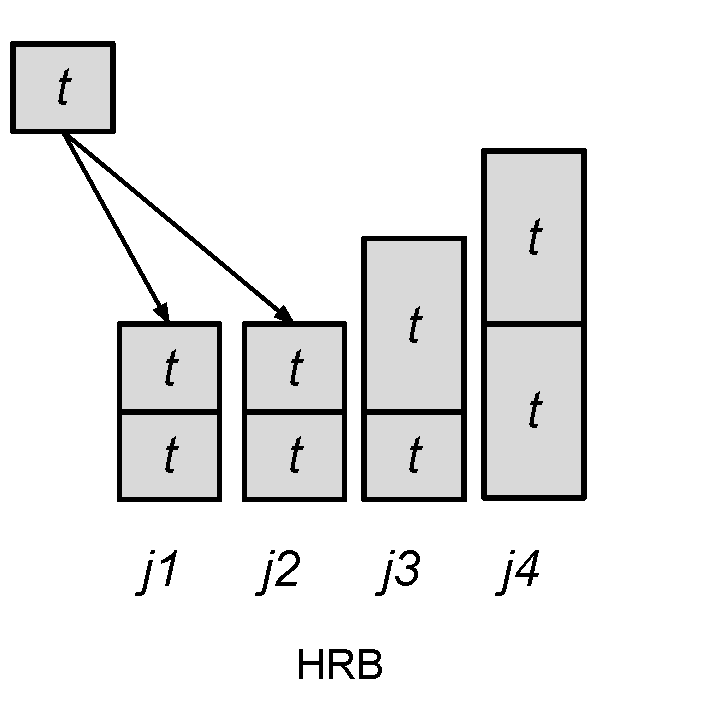
\includegraphics[width=0.5\linewidth]{figure/algorithm_hrb.pdf}
	\caption{An example of HRB.}
	\label{fig:algorithm_hrb}
	\vspace{-10pt}
\end{figure}

However, HRB may cause a Dependency Imbalance problem since the clustering does not take data dependency into consideration. To address this problem, we propose the \textbf{Horizontal Impact Factor Balancing} (HIFB) and the \textbf{Horizontal Distance Balancing} (HDB) methods. 

In HRB, candidate jobs are sorted by their runtime, while in HIFB jobs are first sorted based on their similarity of $IF$, then on runtime. For example, in Fig.~\ref{fig:algorithm_hifb}, assuming 0.2, 0.2, 0.1, and 0.1 IF values of $j_1$, $j_2$, $j_3$, and $j_4$ respectively, HIFB selects a list of candidate jobs with the lowest IF value, i.e. $j_3$ and $j_4$. Then, HRB is performed to select the shortest job ($j_3$). 

\begin{figure}[htb]
	\centering
	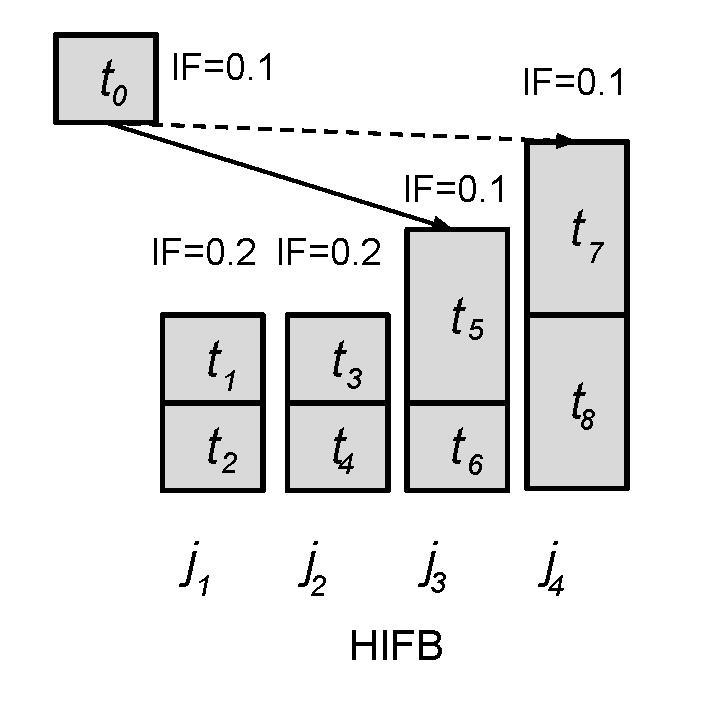
\includegraphics[width=0.5\linewidth]{figure/algorithm_hifb.pdf}
	\captionof{figure}{An example of HIFB.}
	\label{fig:algorithm_hifb}
	\vspace{-10pt}
\end{figure}

Similarly, in HDB jobs are sorted based on the distance between them and the targeted task, then on their runtimes. For instance, in Fig.~\ref{fig:algorithm_hdb}, assuming 2, 4, 4, and 2 the distances to $j_1$, $j_2$, $j_3$, and $j_4$ respectively, HDB selects a list of candidate jobs with the minimal distance ($j_1$ and $j_4$). Then, HRB is performed to select the shortest job ($j_1$). 

\begin{figure}[htb]
	\centering
	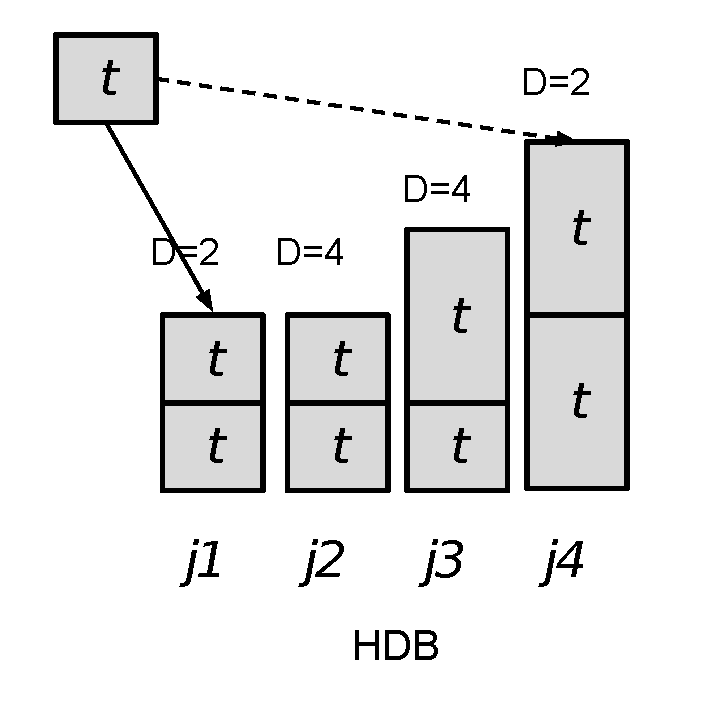
\includegraphics[width=0.5\linewidth]{figure/algorithm_hdb.pdf}
	\captionof{figure}{An example of HDB.}
	\label{fig:algorithm_hdb}
	\vspace{-10pt}
\end{figure}

In conclusion, these balancing methods have different preference on the selection of a candidate job to be merged with the targeting task. HIFB tends to group tasks that share similar position/importance to the workflow structure. HDB tends to group tasks that are closed to each other to reduce data transfers. Table~\ref{tab:2} summarizes the imbalance metrics and balancing methods presented in this work. 

\begin{figure}[htb]
	\centering
	\begin{tabular}{l|l}
		\hline
		Imbalance Metrics & $abbr.$   \\
		\hline
		Horizontal Runtime Variance & \emph{HRV}   \\ 
		%Pipeline Runtime Variance &{\em PRV}  \\ 
		Horizontal Impact Factor Variance & \emph{HIFV} \\ 
		Horizontal Distance Variance & \emph{HDV}  \\ 
		\hline
		Balancing Methods & $abbr.$  \\
		\hline
		Horizontal Runtime Balancing & HRB   \\ 
		% Vertical Clustering & VC \\ 
		Horizontal Impact Factor Balancing & HIFB\\ 
		Horizontal Distance Balancing & HDB \\ 
		\hline
	\end{tabular}
	\captionof{table}{Imbalance metrics and balancing methods.}
	\label{tab:2}
\end{figure}



% Section
\section{Experiment and Evaluation}
\label{sec:experiments}

The experiments presented hereafter evaluate the performance of our balancing methods in comparison with an existing and effective task clustering strategy named Horizontal Clustering (HC)~\cite{Singh:2008:WTC:1341811.1341822}, which is widely used by workflow management systems such as Pegasus. 

\subsection{Experiment Conditions}

We extended the WorkflowSim~\cite{WorkflowSim} simulator with the balanced clustering methods and imbalance metrics to simulate a distributed environment where we could evaluate the performance of our methods when varying the average data size and task runtime. The simulated computing platform is composed by 20 single core virtual machines (worker nodes), which is the quota per user of some typical distributed environments such as Amazon EC2~\cite{AmazonAWS} and FutureGrid~\cite{FutureGrid}. Each machine has 512MB of memory and the capacity to process 1,000 million instructions per second. Task scheduling is data-aware, i.e. tasks are scheduled to resources which have the most input data available.
%WorkflowSim is a feature-rich toolkit to simulate workflow planning and execution. It provides runtime randomization and multiple task clustering methods that we need. 

Two workflows are used in the experiments: LIGO~\cite{LIGO} inspiral analysis, and Epigenomics~\cite{Epigenome}. 
Both workflows are generated and varied using the WorkflowGenerator\footnote[1]{https://confluence.pegasus.isi.edu/display/pegasus/WorkflowGenerator}. LIGO is composed by 400 tasks and its workflow structure is presented in Fig.~\ref{fig:shape} (top); Epigenomics has about 500 tasks and is structured as showed in Fig.~\ref{fig:shape} (bottom). Runtime (average and task runtime distribution) and overhead (workflow engine delay, queue delay, and network bandwidth) information were collected from real traces production environments~\cite{Chen, Juve2013}, then used as input parameters for the simulations.

%We first collected runtime information  (i.e., average and distribution of task runtime) and overhead information (including workflow engine delay, queue delay and network bandwidth) from the real traces that were run on real environments before. 
%Part of runtime distribution and overhead information were shown in \cite{Juve2013} and \cite{Chen} respectively. 
%Then we input these parameters into WorkflowSim and run these workflows repeatedly until the variance is less than 5\% of the average workflow runtime. 

\begin{figure}[htb]
	\centering
	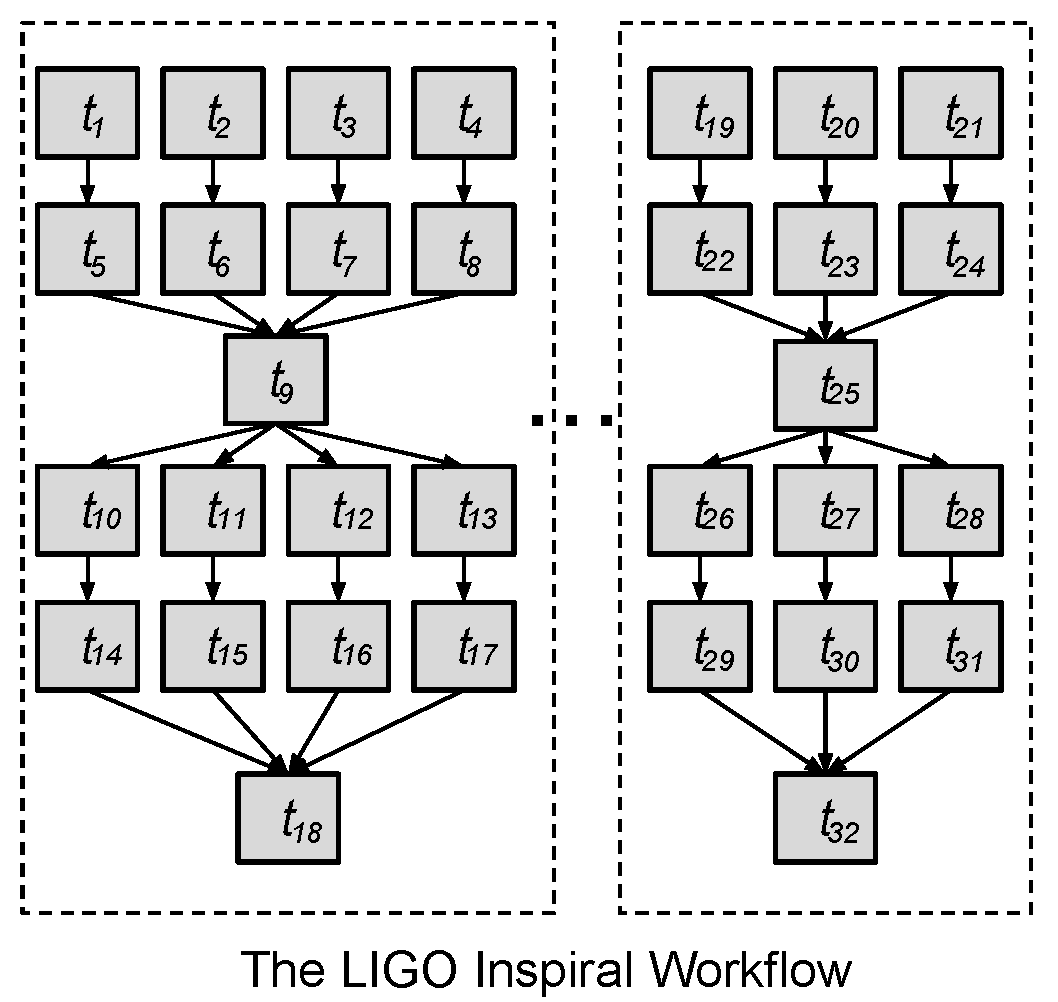
\includegraphics[width=0.65\linewidth]{figure/shape_of_inspiral.pdf} \\
	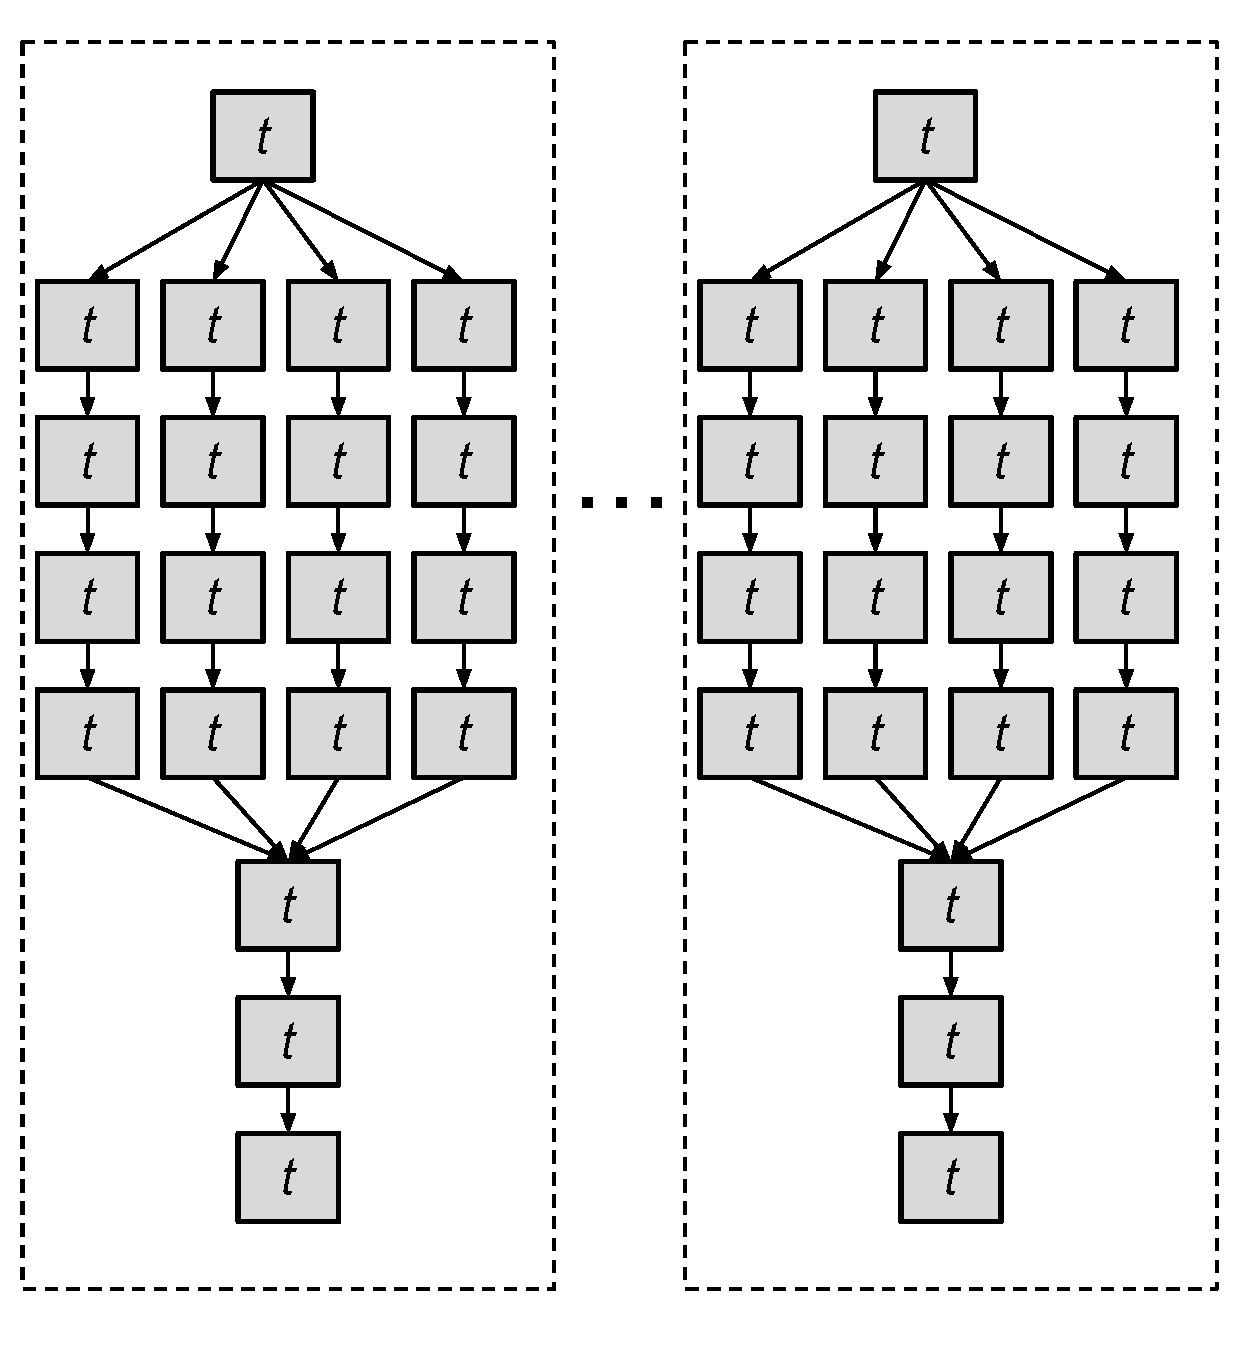
\includegraphics[width=0.7\linewidth]{figure/shape_of_genome.pdf}
	\caption{A simplified visualization of the LIGO Inspiral workflow (top) and Epigenomics workflow (bottom).}
	\label{fig:shape}
	\vspace{-10pt}
\end{figure}

Three sets of experiments are conducted. Experiment 1 aims at determining an appropriate \emph{clustering factor} such that both the workflow runtime performance and the reliability over the dynamic system variation are improved. We randomly select 20\% from LIGO workflow tasks and increase their task runtime by a factor of \emph{Ratio} to simulate the system variation in a production environment.

Experiment 2 evaluates the reliability and the influence of average data size in our balancing methods, since data has becoming more and more intensive in scientific workflows~\cite{Juve2013}. In this experiment set, there is no runtime variance ($HRV = 0$). The original average data size (both input and output data) of the LIGO workflow is about 5MB, and of the Epigenomics workflows is about 45MB. We increase the average data size up to 5GB.

Experiment 3 evaluates the influence of the runtime variation (\emph{HRV}) in our balancing methods. We assume a normal distribution to vary task runtimes based on average and standard deviation. In this experiment set, there is no variation on the data size.

Simulation results present a confidence level of 95\%. We define the performance gain over HC ($\mu$) as the performance of the balancing methods related to the performance of Horizontal Clustering (HC). Thus, for values of $\mu > 0$ our balancing methods perform better than the HC method. Otherwise, the balancing methods perform poorer.

\subsection{Results and Discussion}

Experiment 1: Fig.~\ref{fig:shc} shows the speedup of Horizontal Clustering (HC) for different \emph{Ratio} and \emph{clustering factors}.  We use the speedup of HC in overall runtime compared to the original overall runtime without clustering. The speedup decreases with the increase of the \emph{clustering factor}. However, a smaller \emph{clustering factor} performs worse when the \emph{Ratio} is high. For simplicity, we use $clustering~factor=2$ in the experiments conducted in this work. 

\begin{figure}[htb]
	\centering
	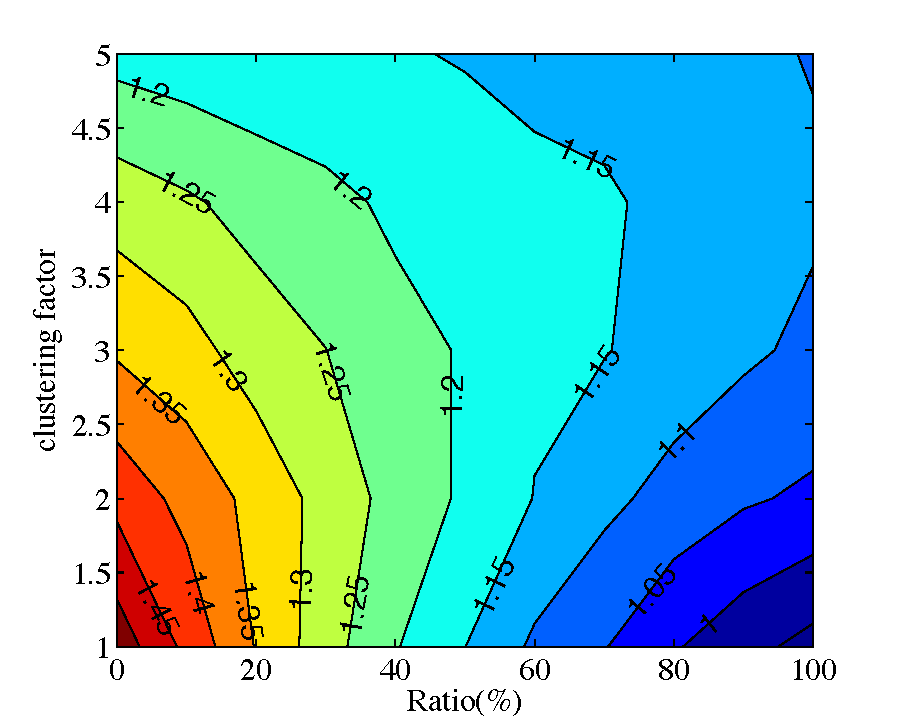
\includegraphics[width=0.8\linewidth]{figure/cfactor.pdf}
	\caption{Experiment 1: Speedup of Horizontal Clustering (HC).}
	\label{fig:shc}
	\vspace{-10pt}
\end{figure}

Experiment 2: Fig.~\ref{fig:performance} (top) shows the performance $\mu$ of the balancing methods compared to the HC method for the LIGO workflow. HIFB and HDB significantly increase the performance of the workflow execution. Both strategies capture the structural and runtime information, reducing data transfers between tasks, while HRB focuses on runtime distribution, which in this case is none. Fig.~\ref{fig:performance} (bottom) shows the performance of the balancing methods for the Epigenomics workflow. When increasing the average data size, only HDB demonstrates significantly improvement related to HC. Investigating the structure of the Epigenomics workflow (Fig.~\ref{fig:shape}-bottom), we can see that all the tasks at the same horizontal level share the same IFs ($HIFV$ = 0), because each branch (surrounded by dash lines) happen to have the same amount of pipelines. Therefore, HIFB has no performance improvement when compared to HC. However, for LIGO (Fig.~\ref{fig:shape}-top), $HIFV \neq 0$, thus HIFB improves the workflow runtime performance.  
%The intuition behind this difference between HDB and HIFB is that 
HDB captures the strong connections between tasks (data dependencies) and HIFB captures the weak connections (similarity in terms of structure). In both workflows, $HDV$ is not zero thus HDB performs better than HC. 

% It is clear that with the increase of the average data size, both HDB and HIFB perform better than HRB. The reason is that both HDB and HIFB can capture the structural information and runtime information, while HRB only focuses on runtime distribution but in this case there is no runtime variance at the horizontal level. 

\begin{figure}[htb]
	\centering
	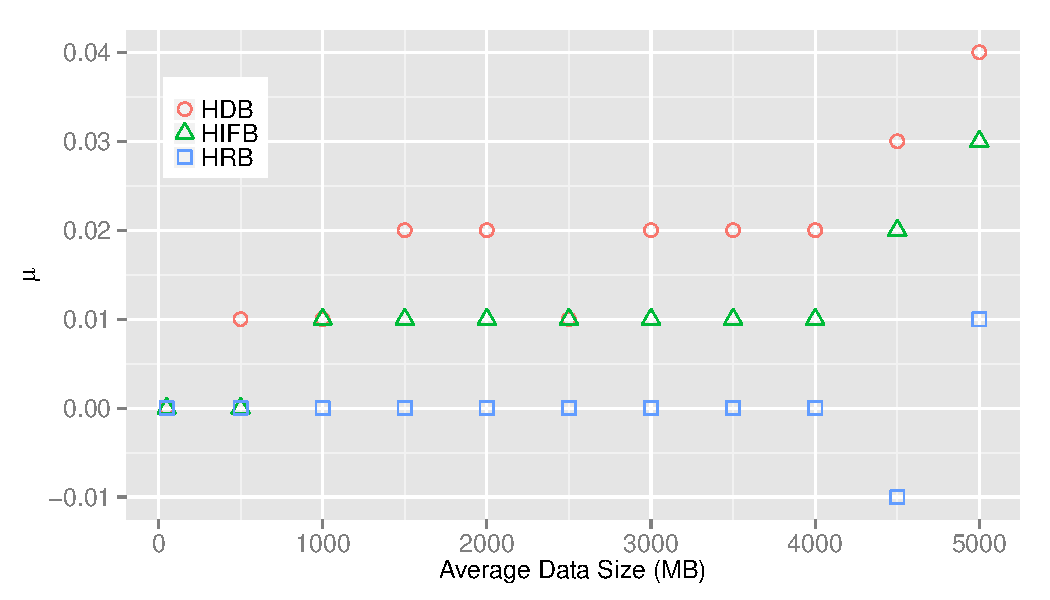
\includegraphics[width=\linewidth]{figure/exp2_ligo.pdf}
	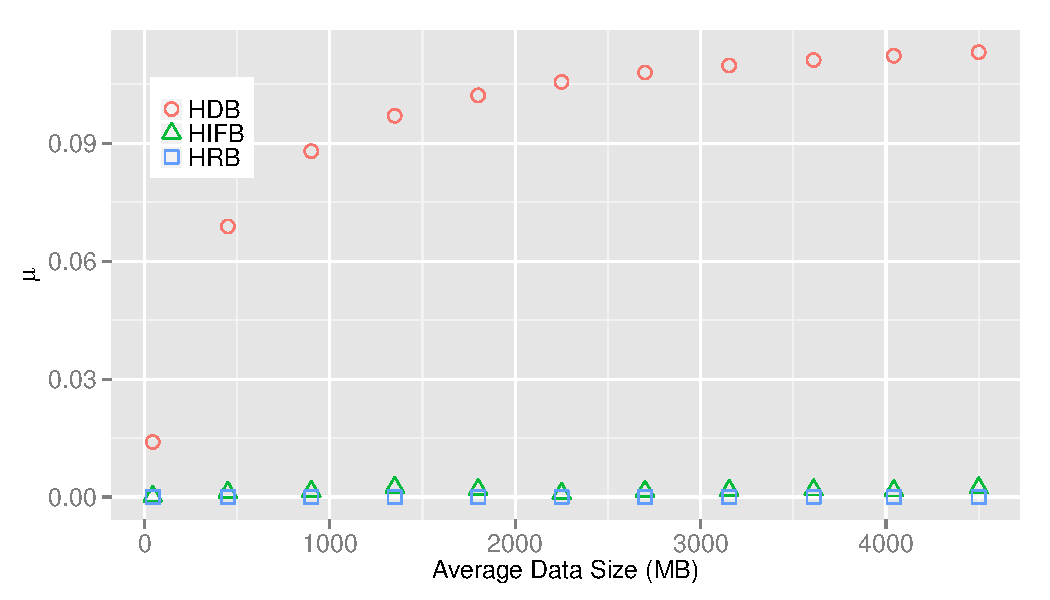
\includegraphics[width=\linewidth]{figure/exp2_genome.pdf}
	\caption{Experiment 2: Performance of the LIGO workflow (top) and the Epigenomics workflow (bottom).}
	\label{fig:performance}
	\vspace{-10pt}
\end{figure}

Experiment 3: Fig.~\ref{fig:incluence_of_hrv} shows the performance gain $\mu$ when varying task runtimes for the LIGO workflow. As expected, when $HRV$ increases HRB over performs HC. However, HDB and HIFB demonstrate poor performance because they merge tasks based on data dependencies first, and then, they balance the runtime distribution. 
For high values of $HRV$, we just simply need to use HRB. Otherwise, we can use either HDB or HIFB while in some cases HIFB fails to capture the structural information. 

\begin{figure}[htb]
\centering
	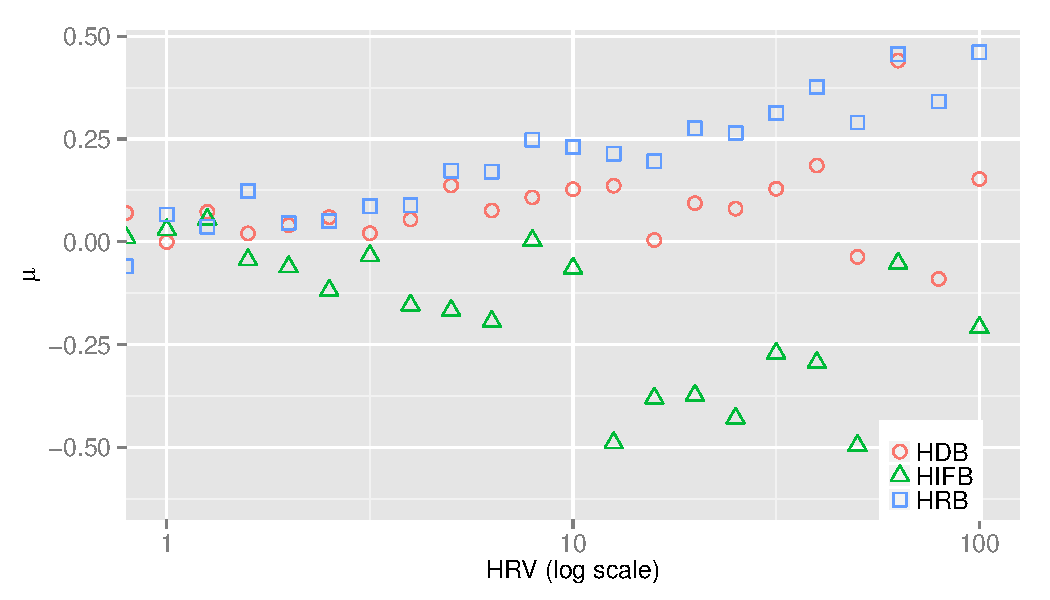
\includegraphics[width=\linewidth]{figure/exp3.pdf}
	\caption{Experiment 3: Influence of $HRV$ (LIGO workflow).}
	\label{fig:incluence_of_hrv}
	\vspace{-10pt}
\end{figure}


% Section
\section{Conclusion}

We presented three balancing methods to address the load balance problem when clustering workflow tasks. We defined three imbalance metrics to quantitative measure workflow characteristics based on task runtime variation (HRV), task impact factor (HIFV), and task distance variance (HDV).

The balanced clustering methods were implemented in the WorkflowSim simulator. Three experiments were conducted using two real workflows. The first experiment showed the gain of task clustering by using a naive horizontal clustering technique. Results showed that our balancing methods can significantly reduce the runtime and data dependency imbalance. For high HRV values, a runtime variance based approach (HRB) performs best over a naive horizontal clustering algorithm. When data dependency is more important HIFB and particularly HDB methods perform better than the naive approach, while HRB performs similarly.
%In this paper, we have proposed three imbalance metrics to evaluate the imbalance problem of a workflow and three balancing methods to address this problem. The experimental results show that our balancing methods can reduce the runtime imbalance and dependency imbalance problem respectively. HRB specially addresses the runtime imbalance problem but does not work well with dependency imbalance problem. HIFB and particularly HDB work well with dependency balancing but does not perform well with the increase of runtime variance. 
In our future work, we will explore the influence of different overheads, and how the HDB method can be extended to perform vertical clustering, i.e. multiple levels clustering.
%We also plan to evaluate more types of workflows. 
%We will also try to dynamically vary the {\em clustering factor} so as to achieve a better performance.
%are worth further discussion. The relationship between these metrics and methods are also discussed.


\bibliographystyle{IEEEtran}
\bibliography{IEEEabrv,biblio}


\end{document}

